\subsection{Deduplication performance analysis} % just find the problem and benefit
\label{sec:background}

%\paragraph{Deduplication for improving storage capacity.}

On-cloud global deduplication software is widely adopted by cloud enterprises for reducing cloud storage consumption and overall storage cost. 
For example, StorReduce~\cite{storReduce}, the deduplication software used by
Google cloud and AWS, 
performs in-line transparent data deduplication. 
%StorReduce resides between the client's application and the hosting cloud storage.
%A number of deduplication methods focus on client-side data deduplication to ensure that only unique files are uploaded, 
%to save network bandwidth, by having the client send a duplicate check request~\cite{xxx}~\cite{xxx}. 
%For example, xxxx\NZ{Hadeel, can you add one example and few relatedwork citation?}. 
Intuitively, such deduplication techniques can be leveraged to eliminate redundant data from the Docker image storage system.  
Except, the Docker image dataset is not amenable to deduplication 
as the images are \emph{compressed archival files}.
%Intuitively, registries can be deployed as a proxy cache to host frequently requested layers to speedup image pulls and improve performance 
%while the backend cloud storage can leverage deduplication to save storage space.
%However, there are several unique problems concerning the integration of caching and deduplication to the unique Docker registries workload: \textbf{compressed layers}. 
%We investigate the potential for data reduction in the Docker registry by estimating the efficacy of layer sharing and file-level deduplication.
%We noticed that the number of public repositories is constantly increasing with a growth that amounts 
%to around 1 million repositories annually. 
%This corresponds to~130\,TB of annual growth in storage needs 
%\HA{but it is actually less because of shared layers, right?}, 
%costing around~\$15,000 a month if Google Cloud Storage is used~\cite{GoogleCloudStoragePricing}.
%This growth implies significant benefits to data deduplication. 


As discussed in~\cref{sec:intro}, only $3$\% of the files in a sample Docker hub image collection were found to be unique, mainly becuase 
 compressed files have a very low deduplication ratio~\cite{meister2012study}.
Thus, 
we can realize significant space savings if we can remove the 
duplicate files. This entails decompressing files before performing deduplication, and collecting components of layers from multiple servers.
%
To quantify the performance overhead of such an approach involving decompressing, deduplication, and then re-compressing,
we setup five registry instances. Each instance has a local file system as their backend storage system. We
implemented file-level deduplication with decompression and compression operations.
We replayed the IBM registry workload \texttt{Dal}~\cite{dockerworkload} 
%by sending requests randomly 
randomly to our five registries and measured the latency. 
%
Figure~\ref{fig:avg_latency_dedup_nodedup} shows the average latency observed 
across five registries.
%\arb{average across what??}\NZ{addressed}.
Note that since 
%the IBM registry workload 
\texttt{Dal} does not contain real layers,
we extract the layer digest from each request and match it with a layer randomly selected from our Docker Hub dataset to emulate realistic requests.

Without deduplication,
the average latency for requesting a layer is about $2$~s for layers with sizes $\textless50$~MB.
The latency increases to $12$~s when the above deduplication is implemented in the backend storage system.
Furthermore, Docker registry performance drops down dramatically for larger layers.
We observe that the average latency for requesting layers $\textgreater50$~MB and $\textless1$~GB
is about $128$~s. The latency worsens with dedupliation to on average of about $800$~s.
%\NZ{todo:graph: less than, }
%\HA{running five registries, replaying dal trace using trace replayer-cite, and since the replayer doesn't use real layers we randomly match the request to our dataset downloaded from docker hub. describe how we got these numbers. for dedup, we simply implemented a decompress/compress + file-level deduplication on backend storage systems, we use a CHT based distributed storage system. Figure~\ref{fig:avg_latency_dedup_nodedup}}
\begin{figure}[t]
	\centering
	%\scriptsize
	\begin{minipage}{0.225\textwidth}
		\centering
		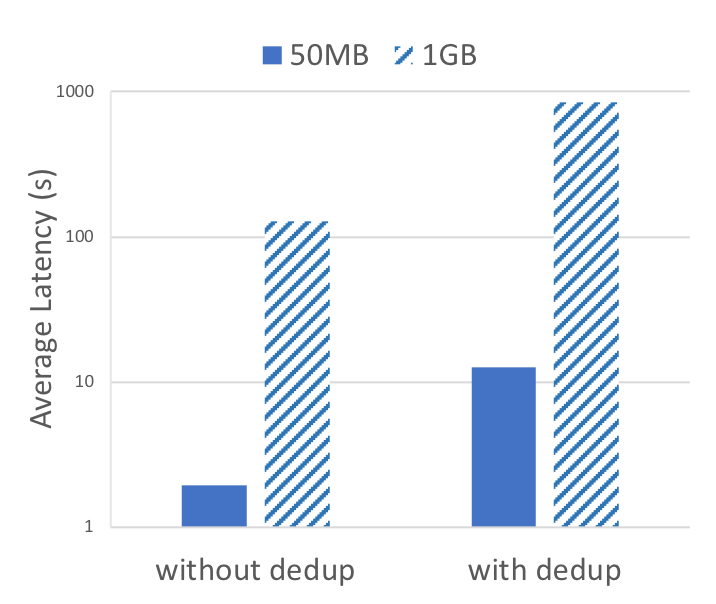
\includegraphics[width=1\textwidth]{graphs/avglatency_dedup_nodedup.png}
		\caption{Average latency.}
		\label{fig:avg_latency_dedup_nodedup}
	\end{minipage}
	\begin{minipage}{0.225\textwidth}
		\centering
		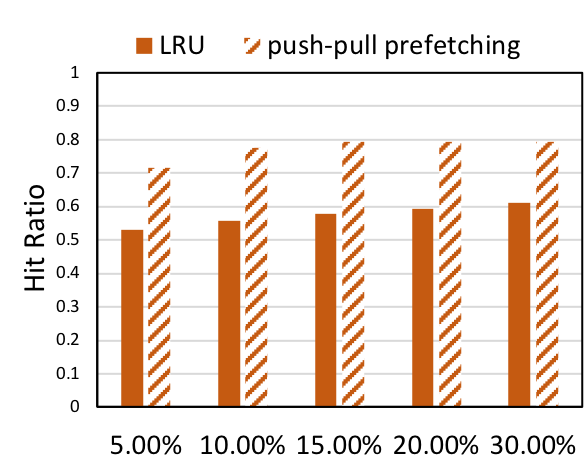
\includegraphics[width=1\textwidth]{graphs/lru_prefetch_hits.png}
		\caption{Hit ratio.}
		\vspace{-3pt}
		\label{fig:lru_prefetching_hits}
	\end{minipage}
\end{figure}
% for LRU and push-pull prefetching under different cache sizes (\% of total accessed layers).

